

\section{Methodology}
\label{sec:SIMPOR_method}
To alleviate the negative effects of data imbalance, we propose a comprehensive approach, \MethodnameLong{} (\Methodname), which aims to generate synthetic samples for minority classes. First, the informative region that contains informative samples is determined and balanced by creating surrounding synthetic neighbors for minority samples. The remaining region is then fully balanced by arbitrarily generating minority samples' neighbors. The remainder of this section provides further information about how our approach was developed.  

\subsection{Methodology Motivation}  
As Chazal and Michel mentioned in their work \cite{leroueil_compressibility_1996}, the natural way to highlight the global topological structure of the data is to connect data points' neighbors; our proposed method aligns with their observation by generating surrounding synthetic neighbors for minority samples to preserve data topology. Thus, our technique not only generates more data for minority class but also preserve the underlying topological structure of the entire data. 

Similar to \cite{ertekin_learning_2007} and \cite{aggarwal_active_2020}, we believe that informative samples play the most important role in the prediction success of both traditional machine learning models (e.g., SVM, Naive Bayes) and modern deep learning approaches (e.g., neural network). Thus, our technique finds these informative samples and focuses on augmenting minority data in this region. In this work, an entropy-based active learning strategy mentioned in \ref{sec:EAL} is applied to find the samples that contain more information to the model. This strategy is perhaps the most popular active learning technique and over-performs many other techniques on several datasets \cite{DAL}, \cite{7393573} \cite{settles_analysis_2008}.

\subsection{Generating minority synthetic data}  
\label{sec:solvingOptimization}
\Copy{1.1a}{
A synthetic neighbor $ x'$ and its label $y'$ can be created surrounding a minority sample $x$ by adding a small random vector $v$ to the sample, $x' = x + v$. Thus, $x'$ can be selected on the d-sphere's surface centered at $x$ with a radius of $|\vec{v}|$. For notation convenience, let $r = |\vec{v}|$ be the radius of the d-sphere. To enrich the synthetic samples, $r$ is sampled from a defined Gaussian distribution to generate a new synthetic sample distance each time. This section describes how the direction and distance of a synthetic sample are determined, which can also be represented via the direction and length of vector $\vec{v}$.

It is critical to generate synthetic data in the informative region because synthetic samples can unexpectedly jump across the decision boundary. This can be harmful to models as this might create outliers and reduce the model's performance. Therefore, we safely find vector $\vec{v}$ towards the minority class, such as $\vec{v}_0$ and $\vec{v}_1$ depicted in Figure \ref{fig:problem}.} Our technique is described via a binary classification scenario as follows. 

Let's consider a binary classification problem between majority class A and minority class B. 
From the Bayes' theorem, the posterior probabilities $p(y'=A|x')$ or $p(y'=B|x')$ can be used to present the probabilities that a synthetic sample $x'$ belongs to class A or class B, respectively. Let the two posterior probabilities be $f_0$ and $f_1$; they can be expressed as follows. 
\begin{align}
	\label{eq:posterior}
	p(y'=A|x') = \frac{p(x'|y'=A)\:p(A)}{p(x')} = f_0 \\
	p(y'=B|x') = \frac{p(x'|y'=B)\:p(B)}{p(x')} = f_1  
\end{align}

As mentioned earlier, each synthetic data $x'$ is generated so that it maximizes the probability of $x'$ belonging to the minority class $B$ and minimizes the chance $x'$ falling into the majority class $A$. Thus, a technique that maximizes the fractional posterior $f$ is proposed,   
\begin{align}
	\label{eq:fracpost}
	f &= f_1/f_0  \\
	&=\frac{p(x'|y'=B) \:p(B)}{p(x'|y'=A) \: p(A)}. \label{equ:f_ratio}
\end{align}


\textbf{\textit{Approximation of likelihoods in Equation \ref{equ:f_ratio}:}} A non-parametric kernel density estimates (KDE) is selected to approximate the likelihoods $p(x'|y'=A)$ and $p(x'|y'=B)$ as KDE is flexible and does not require specific assumptions about the data distribution. One can use a parametric statistical model such as Gaussian to approximate the likelihood; however, it oversimplifies the data and does not work effectively with topological complex data, especially in high dimensions. In addition, parametric models require an assumption about the distribution of data which is difficult in real-world problems since we usually do not have such information. On the other hand, KDE only needs a kernel working as a window sliding through the data. Among different commonly used kernels for KDE, we choose Gaussian Kernel as it is a powerful continuous kernel that would also eases the derivative computations for finding optima.
 
\Copy{PriorApproximation}{
\textbf{\textit{Approximation of priors in Equation \ref{equ:f_ratio}:}} Additionally, we estimate the prior probabilities of observing samples in class A ($p(A)$) and class B ($p(B)$) (in Equation \ref{equ:f_ratio}) by the widely-used Empirical Bayes Method \cite{empiricalBayes} to leverage the existing information from the original data. The estimates are denoted as $\widehat{p(A)}$ and $\widehat{p(B)}$ respectively.

\textbf{\textit{Equation \ref{equ:f_ratio} Approximation:} } Let $X_A$ and $X_B$ be the subsets of dataset $X$ which contain samples of class A and class B, $X_A=\{x: y=A  \}$ and $X_B=\{x: y=B  \}$. $N_A$ and $N_B$ are the numbers of samples in $X_A$ and $X_B$. $d$ is the number of data dimensions. $h$ presents the width parameter of the Gaussian kernel. The posterior ratio for each synthetic sample $x'$ then can be estimated as follows:

\begin{align}
	\label{eq:fracpost_estimation}
	f &= \frac{p(x'|y'=B)  \: p(B)}{p(x'|y'=A) \: p(A)} \\
	&\propto \frac{ \frac{1}{N_B h^d} \: \sum_{i=1}^{N_B}{ (2\pi)^{-\frac{d}{2}} \: e^{\frac{1}{2}{(\frac{x'-X_{B_i}}{h})^2} } } \: \widehat{p(B)} }
	{ \frac{1}{N_A h^d} \:  \sum_{j=1}^{N_A}{ (2\pi)^{-\frac{d}{2}} \: e^{ \frac{1}{2} {(\frac{x-X_{A_j}}{h})^2} } }\: \widehat{p(A)} }\\
	& \propto \frac{ \frac{1}{N_B h^d} \: \sum_{i=1}^{N_B}{ \: e^{\frac{1}{2}{(\frac{x'-X_{B_i}}{h})^2} } } \: \widehat{p(B)} }
	{ \frac{1}{N_A h^d} \:  \sum_{j=1}^{N_A}{  \: e^{ \frac{1}{2} {(\frac{x-X_{A_j}}{h})^2} } }\: \widehat{p(A)} }
	\label{equ:f}
\end{align} 
}


\textbf{\textit{Selecting bandwidth parameter $h$ for Gaussian kernel:} } The bandwidth is automatically selected for each dataset using the most common method, namely Scott's rule of thumb, proposed by Scott \cite{scott_2015}. With an attempt to minimize the mean integrated squared error, the parameter is estimated as $h = N^{(-\frac{1}{d+4})}$ where $N$, $d$ are the number of data points and the number of dimensions respectively. This study utilizes a scikitlearn python library for KDE, including bandwidth selection. The implementation detail can be found at \cite{skitlearnKDE}. 

\textbf{\textit{Finding synthetic samples surrounding a minority sample:}} To generate neighbors for each minority sample that maximizes Function \text{f} in Equation \ref{equ:f}, points on each $r$-radius sphere centered at a minority sample are considered synthetic instances. As a result, a vector $\vec{v}$ can be added to a minority sample for generating a new instance. \Copy{1.1b}{The relationship between a synthetic sample $x'$ and a minority sample can be described as follows,
\begin{align}
	\label{equ:vecV}
	\vec{x'} =  \vec{x} + \vec{v},
\end{align}
where the length of $\vec{v}$ is equal to $r$, and $r$ is sampled from a Gaussian distribution,
\begin{align}
     r \sim \mathcal{N}(0,\,(\alpha R)^{2}),
     \label{equ:r_dist}
\end{align}
where $\alpha R$ is the standard deviation of the Gaussian distribution and $ 0< \alpha <=1 $.
The range parameter $R$ is relatively small and computed as the average distance of a minority sample $x$ to its k-nearest neighbors. This will ensure that the generated sample will surround the minority sample. The Gaussian distribution with the mean of zero and the standard deviation $\alpha R$ controls the distance between the synthetic samples and the minority sample. The standard deviation is tuned from 0 to R by a coefficient $\alpha \in (0,1]$. The larger the $\alpha$ is, the farther synthetic data is placed from its original sample.} Consider a minority sample $x$ and its k-nearest neighbors in the Euclidean space, $R$ can be computed as follows:

\begin{align}
	R = \frac{1}{k}\sum\limits_{1}^{k} ||x-x_j ||,
\end{align}
where $||x-x_j||$ is the Euclidean distance between a minority sample $x$ and its $j$th neighbor. $k$ is a parameter indicating selected number of neighbors. 


\begin{figure}[th]
	%[trim=left bottom right top, clip]
	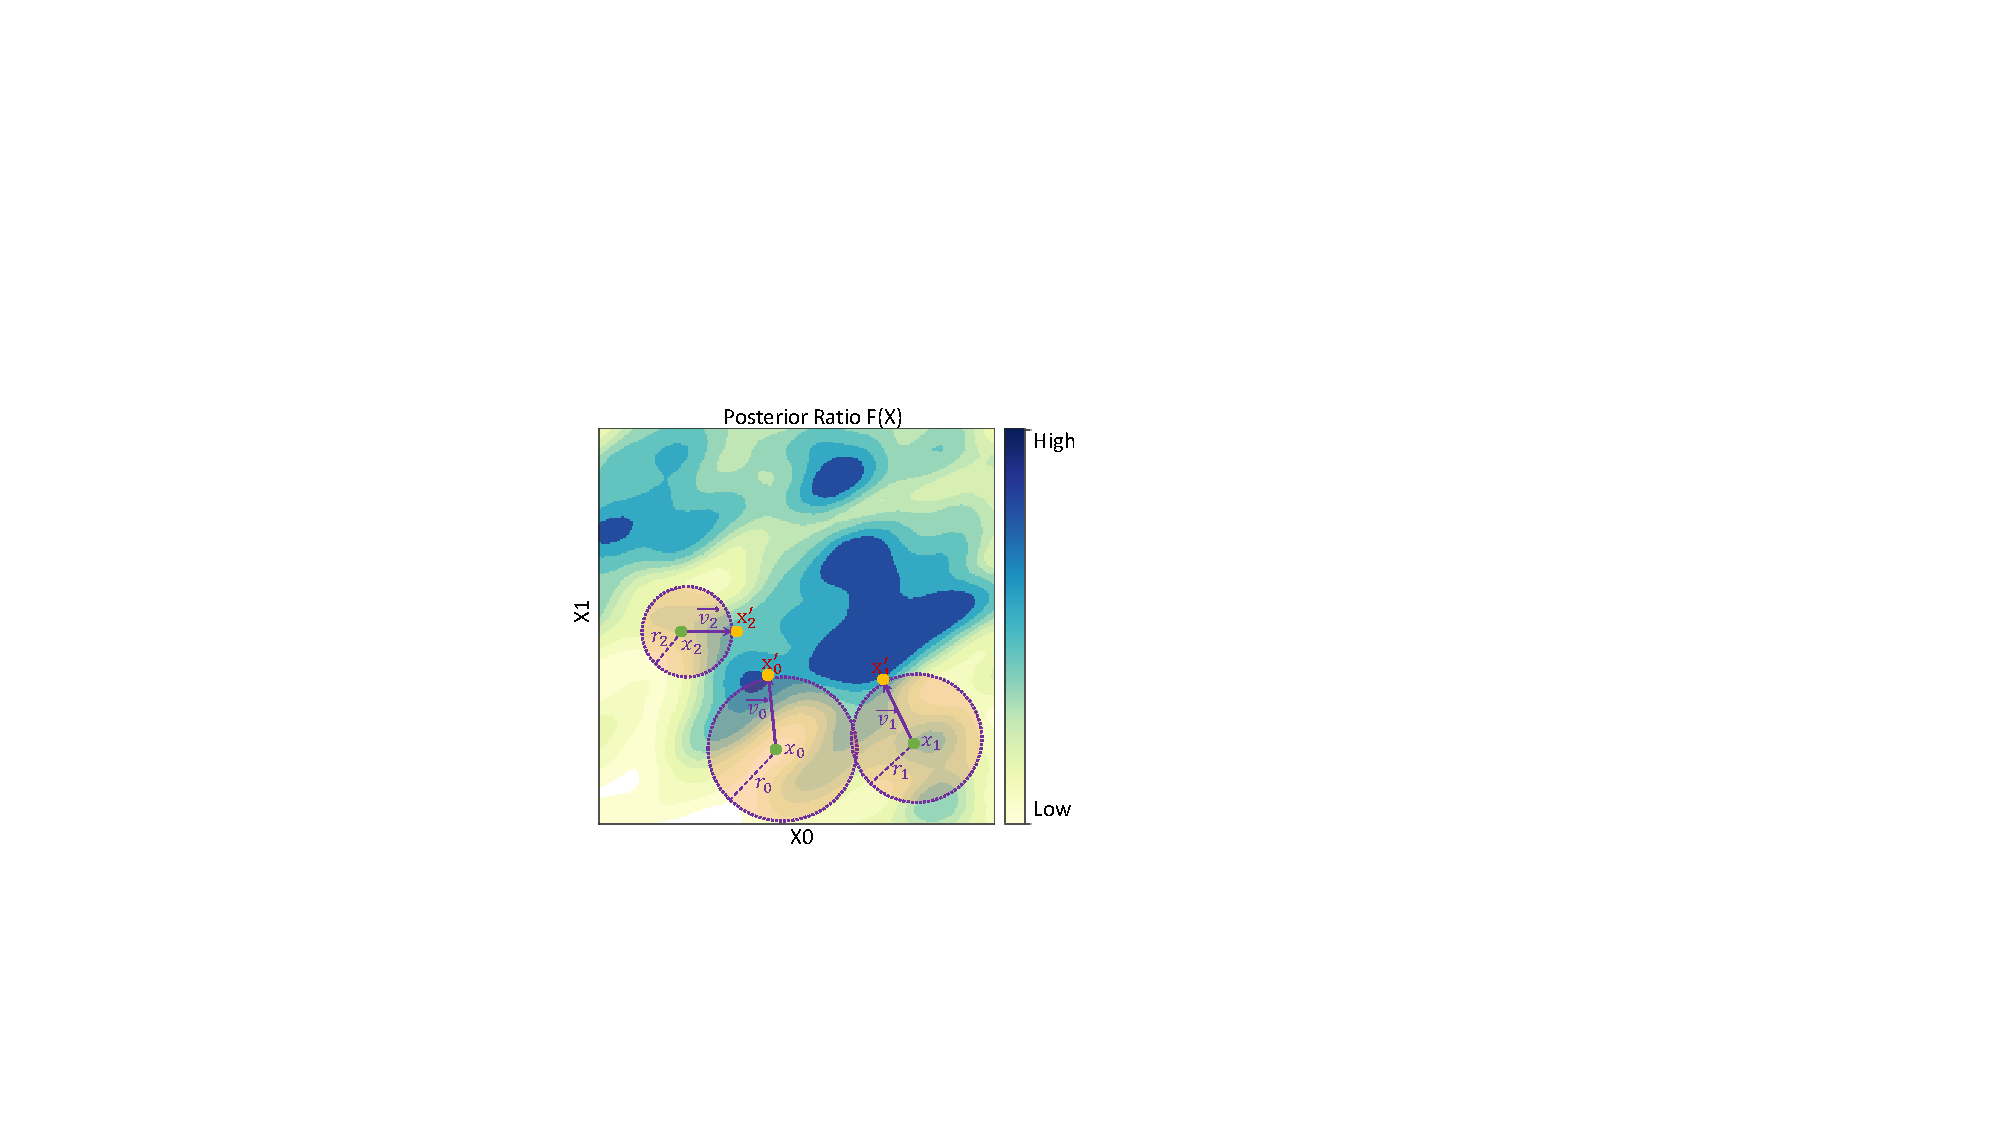
\includegraphics[width=\linewidth, trim=240 120 390 160,clip]{Figures/MaxPosteriorRatio/sphere_maxF.pdf}
	\caption{Demonstration on how \Methodname{} generates three synthetic samples $x'_0, x'_1, x'_2$, from three minority samples $x_0, x_1, x_2$, by maximizing the Posterior Ratio. }
	\label{fig:sphere_maxF}
\end{figure}

Figure \ref{fig:sphere_maxF} depicts a demonstration of finding 3 synthetic samples from 3 minority samples. In practice, one minority can be re-sampled to generate more than one synthetic samples. For a minority sample $x_0$, we find a synthetic sample $x_0'$ by maximizing the objective function $f(x_0'), x_0' \in X$ with a constraint that the Euclidean length of $\vec{v_0}$ equals to a radius $r_0$, $||\vec{v_0}|| = r_0$ or $||\vec{x_0'}-\vec{x_0}||=r_0$ (derived from Equation \ref{equ:vecV}). 


The problem can be described as a constrained optimization problem. For each minority sample $x$, we find a synthetic sample $x'\in \mathbb{R}^d$ lying on the d-sphere centered at $x$ with radius $r$ and maximizing function in Equation \ref{equ:f},
\begin{align}
	\label{prob:optimazation}
	\max_{x'} {f(x')} \;\;\; \textrm{s.t.}\; ||\vec{x'} - \vec{x}||=r.
\end{align}

\textbf{\textit{Solving optimization problem in Equation \ref{prob:optimazation}:}} Interestingly, the problem in Equation\ref{prob:optimazation} can be solved numerically. Function $f(x)$ in Equation \ref{equ:f} is defined and continuous for $x' \in (-\infty, +\infty)$ because all of the exponential components (Gaussian kernels) are continuous and greater than zero. In addition, the constraint, $||\vec{x'} - \vec{x}||=r$, which contains all points on the sphere centered at $x$ with radius $r$ is a closed set (\cite{wikipedia_2021}). Thus, a maximum exits as proved in \cite{maximum_exist}. To enhance the diversity of synthetic data, either the global maximum or any local maximum can be accepted so that the synthetic samples will not simply go to the same direction.  

We solve the problem in Equation \ref{prob:optimazation} by using the Projected Gradient Ascent approach in which we iteratively update the parameter to go up the gradient of the objective function. A local maximum is found if the objective value cannot be increased by any local update. For simplification, we rewrite the problem in Equation \ref{prob:optimazation} by shifting the origin to the considered minority sample. The problem becomes finding the maximum of function $f(x')$, $x' \in \mathbb{R}^d$, constrained on a d-sphere, i.e., $||x'||=r$. Our solution can be described in Algorithm \ref{alg:optimization}. After shifting the coordinates system, we start by sampling a random point on the constraint sphere (line $1-2$). The gradient of the objective function at time $t$, $g_t(x'_t)$, is computed and projected onto the sphere tangent plane as $p_t$ (line $4-5$). It is then normalized and used for update a new $x'_{t+1}$ by rotating a small angle $lr*\theta$ (line $6-7$). The algorithm stops when the value of $f(x')$ is not increased by any update of $x'$. We finally shift to the original coordinates and return the latest $x'_t$.   



\textbf{\textit{Avoiding synthesis of noise:}} To reduce the chance of misplacing synthetic samples on another class region because of noisy borderline and mislabeled minority samples, we set a policy for rejecting minority candidates which are selected for oversampling. The idea is to reject candidates surrounded mainly by other class samples. More specifically, we count the labels of the candidate's $k$-nearest neighbors and reject this candidate if there exists a class that its' number of samples is greater than the number of the minority samples. For example, the candidate is rejected when a class-A sample is selected for generating synthetic data, and its 5-nearest neighbors contain four class-B samples and one class-A sample. This is to avoid selecting mislabeled samples and noisy borderline samples for oversampling.        

\subsection{Algorithm}
Our strategy can be described in Algorithm \ref{alg:SIMPOR}. The algorithm takes an imbalanced dataset as its input and results in a balanced dataset which is a combination of the original dataset and synthetic samples. We first choose an active learning method $AL(\cdot)$ and find a subset of informative samples $S$ by leveraging entropy-based active learning (lines $1-2$). We then generate synthetic data to balance $S$. For each random sample $x_i^c$ in $S$ and belonging to minority class $c$, we randomly sample a small radius $r$ and find a synthetic sample that lies on the sphere centered at $x_i^c$ and maximizes the posterior ratio in Equation \ref{equ:f} (lines $3-11$). The process is repeated until the informative set $S$ is balanced. Similarly, the remaining region is balanced, which can be described in the pseudo-code from line $12$ to line $20$. The final output of the algorithm is a balanced dataset $D'$.       
